\chapter{2D Segmentation}

In this chapter, we establish the task of 2D Segmentation of EM images, attempt to train models that perform well on this task, and evaluate our results. The purpose of these experiments is not so much to achieve state-of-the-art performance on the task, but to examine the effect that increasing training data quality and reducing variance in predictions has on model performance.

\section{Task Definition}

2D Segmentation involves taking a single 2D slice of EM tissue and segmenting it into its constituent cells. Compared to 3D segmentation, this is a simple task, but will still allow us to show the properties of different models on EM data. To achieve segmentation, we will train models that predict boundaries of cells, and then use a Watershed algorithm to segment based on those boundary predictions.

The problem statement for 2D Boundary detection is such: given a 2-dimensional single-channel (i.e. greyscale) image of neural tissue taken with an electron microscope, produce an image that labels the boundaries of all the distinct cells in the image. An example of this boundary-detection task can be found in Figure \ref{fig:isbi_example}. This task is made somewhat more difficult by the existence of organelles with well-defined borders, as well as blood vessels and structured interstitial tissue.

\begin{figure}
    \centering
	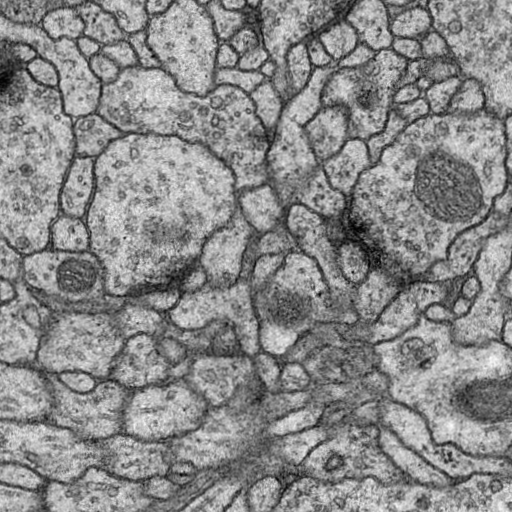
\includegraphics[width=0.33\textwidth]{img/isbi_raw_example}
	\hspace{1cm}
	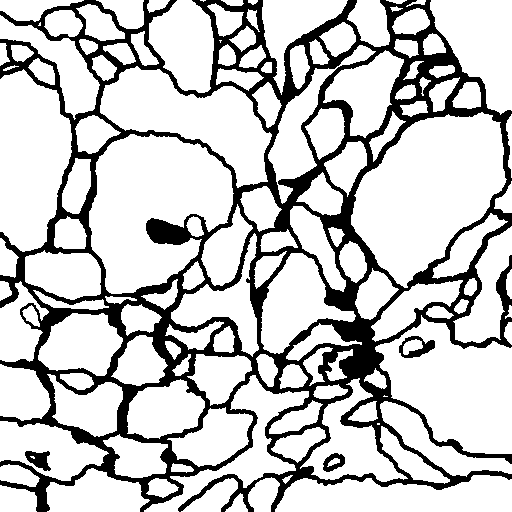
\includegraphics[width=0.33\textwidth]{img/isbi_label_example}
    \caption[An example of 2D boundary detection]{An example of 2D boundary detection. Left: the original image taken with an electron microscope. This particular example is neuron tissue taken from \textit{Droposphila melanogaster} in a dataset created for the ISBI 2012 EM segmentation challenge \cite{Arganda-Carreras2015}. The resolution of each pixel is 4nm x 4nm. Right: The ground truth boundaries corresponding to cell membranes in the input image, as labeled by human experts. The labels are binary values, although the actual border deliniation is somewhat arbitrary due to the fact that real applications of boundary detection are invariant to small differences in boundary shapes.}
    \label{fig:isbi_example}
\end{figure}

\section{Evaluation Metrics}

The two main evaluation metrics we will use for this task are Rand Score and Pixel Error. Formal definitions of both of these error metrics can be found in Appendix A. 

\begin{itemize}
\item \textbf{Rand Score}: We will use the Rand Score to determine whether or not the segmentation process correctly labels different cells as different objects. We will also look at the Rand Split Score and the Rand Merge Score, to see where the models inaccurately split and merge different regions.
\item \textbf{Pixel Error}: We will use the Pixel Error to gauge the efficacy of our models at predicting the intermediate boundary stage.
\end{itemize}

\section{Models}

We define two models - both closely resembling models from the literature -  with which we will run experiments:

\begin{itemize}
\item \textbf{N4} The N4 Architecture is a standard, fully-convolutional network. We use an identical architecture to the architecture outlined in the original N4 paper\cite{Cirean}. The architecture uses comparatively fewer convolutions, each with comparatively larger filter sizes. The number of feature maps stays the same throughout the net, and ends with a fully connected layer to predict an output pixel with a sigmoid function. Intermediate non-linearities are ReLU. Given a large enough input, an entire output patch can be predicted pixel-by-pixel. The effective field-of-view for each pixel in the output is a 95 pixel square in the input image.

\begin{figure}[h]
\centering
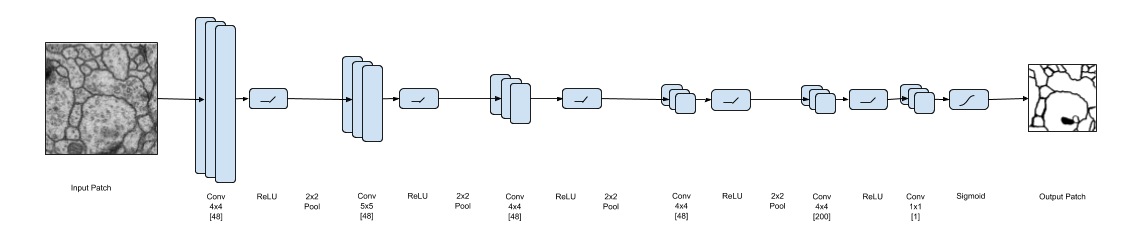
\includegraphics[width=\textwidth]{img/N4.png}
\caption{The N4 architecture used for 2D segmentation}
\label{fig:n4}
\end{figure}

\item \textbf{VD2D} The VD2D Architecture is also a standard, fully-convolutional network, and is nearly identical to the architecture originally used in the VD2D paper\cite{Lee}. By comparison, the VD2D architecture is deeper than N4, and uses more successive layers with smaller convolutional filters. Activations are ReLU, and the output is a pixel affinity. The effective field of view for each pixel in the output is a 109 pixel square in the input image.

\begin{figure}[h]
\centering
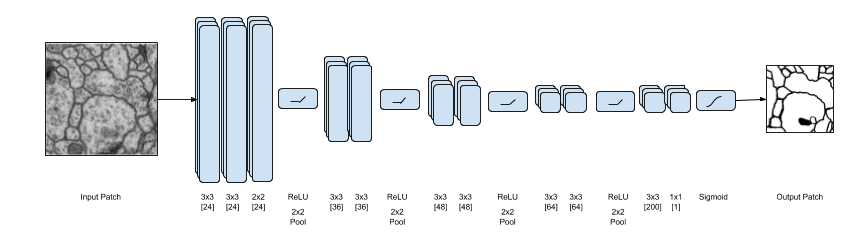
\includegraphics[width=\textwidth]{img/VD2D.png}
\caption{The VD2D architecture used for 2D segmentation}
\label{fig:vd2d}
\end{figure}

\end{itemize}

\section{Dataset}

One prominent competition that evaluates performance on this sort of task is the International Symposium on Biomedical Imaging (ISBI) EM Segmentation Challenge, which has had active submission since 2012. The ISBI Challenge organizers provides a training set of EM images, along with a set of binary boundary maps. The challenge website describes the training data as \quotes{a set of 30 sections from a serial section Transmission Electron Microscopy (ssTEM) data set of the Drosophila first instar larva ventral nerve cord (VNC). The microcube measures 2 x 2 x 1.5 microns approx., with a resolution of 4x4x50 nm/pixel}\cite{Arganda-Carreras2015}. This resolution description implies that each pixel represents a 4x4nm patch on the surface of a slice, with each slice being 50nm thick. We build prediction systems using several different architectures, regularization methods, and data transformation techniques. We make several submissions to the leaderboard, ultimately scoring quite competitively.

The dataset comes with two EM stacks from the same neural tissue: one train stack with boundary labels consisting of (30) 512x512 slices; and one test stack without boundary labels consisting of (30) 512x512 slices. We hold out 25\% of the train stack (7 slices) as a validation set to report results.

\section{Training}

We trained our nets each for 30000 iterations (with the exception of VD2D w/o augmentation, which was trained for 15000), sampling the training set in random patches, in mini-batches of 16. For every model, we sought to minimize the cross entropy between the predicted boundaries and the true boundary labels, defining our loss function as:

$$\mathcal{L}(\bm{x}, \bm{y}) = -\log(\sigma(\bm{y}^{T}\bm{x}-(1-\bm{y}^{T})\bm{x}))$$
where $\sigma$ is the sigmoid function, $\bm{x}$ is the prediction, and $\bm{y}$ is the true boundary.

At each step, we executed one iteration of optimization using the Adam Optimizer, and ever 100 steps we made predictions on the validation set to see how well the model generalized.

We made five different training runs using different parameters:

\begin{itemize}
	\item \textbf{N4, w/o augmentation}: We trained our N4 model on the train data using the procedures above, making sure not to add any data augmentations during the training process.
	\item \textbf{VD2D, w/o augmentation}: We trained our VD2D model on the train data using the procedures above, making sure not to add any data augmentations during the training process.
	\item \textbf{N4}: We trained our N4 model on the train data using the procedures above, this time including data augmentations that randomly flipped, rotated, blurred, and otherwise distorted each sample before being fed into the net.
	\item \textbf{VD2D}: We trained our VD2D model on the train data using the procedures above, this time including data augmentations that randomly flipped, rotated, blurred, and otherwise distorted each sample before being fed into the net.
	\item \textbf{VD2D (x5)} We independently ran 5 iterations of VD2D training (with augmentation), and then used the ensembling technique of model averaging to derive predictions.
\end{itemize}

\section{Results}

After training, we run the trained models on the validation set (since we don't have labels for the test set) to determine their performance. Results are numerically summarized in Table \ref{tab:2d_results}, and graphs of Rand Score and Pixel Error on the validation set over the course of training are displayed in Figure \ref{fig:2d_training_curves}. Of the two models, VD2D generally performed better than N4, models trained with augmentation performed much better than those trained without, and the ensembled VD2D performed the best out of all training runs in terms of Rand Full Score.

\begin{table}
\centering
	\begin{tabular}{lllll}
\toprule
{} & Pixel Error & Rand - Full & Rand - Merge & Rand - Split \\
\midrule
N4 w/o aug   &    0.112204 &     0.65693 &     0.506545 &     0.934315 \\
N4           &   0.0827646 &    0.950296 &     0.933164 &     0.968069 \\
VD2D w/o aug &   0.0998995 &     0.80245 &     0.725266 &     0.898018 \\
VD2D         &   0.0842352 &    0.954286 &     0.976404 &     0.933148 \\
VD2D (x5)    &    0.083214 &    0.975745 &     0.985624 &     0.968843 \\
\bottomrule
\end{tabular}

	\caption[Results of 2D Segmentation]{The results of various architectures on the 2D Segmentation task. Notice that using data augmentation drastically improves the performance of the nets. Additionally, ensembling multiple instances of the best architecture produces the best Rand Score.}
	\label{tab:2d_results}
\end{table}

\begin{figure}
\centering
\textbf{Rand Index}
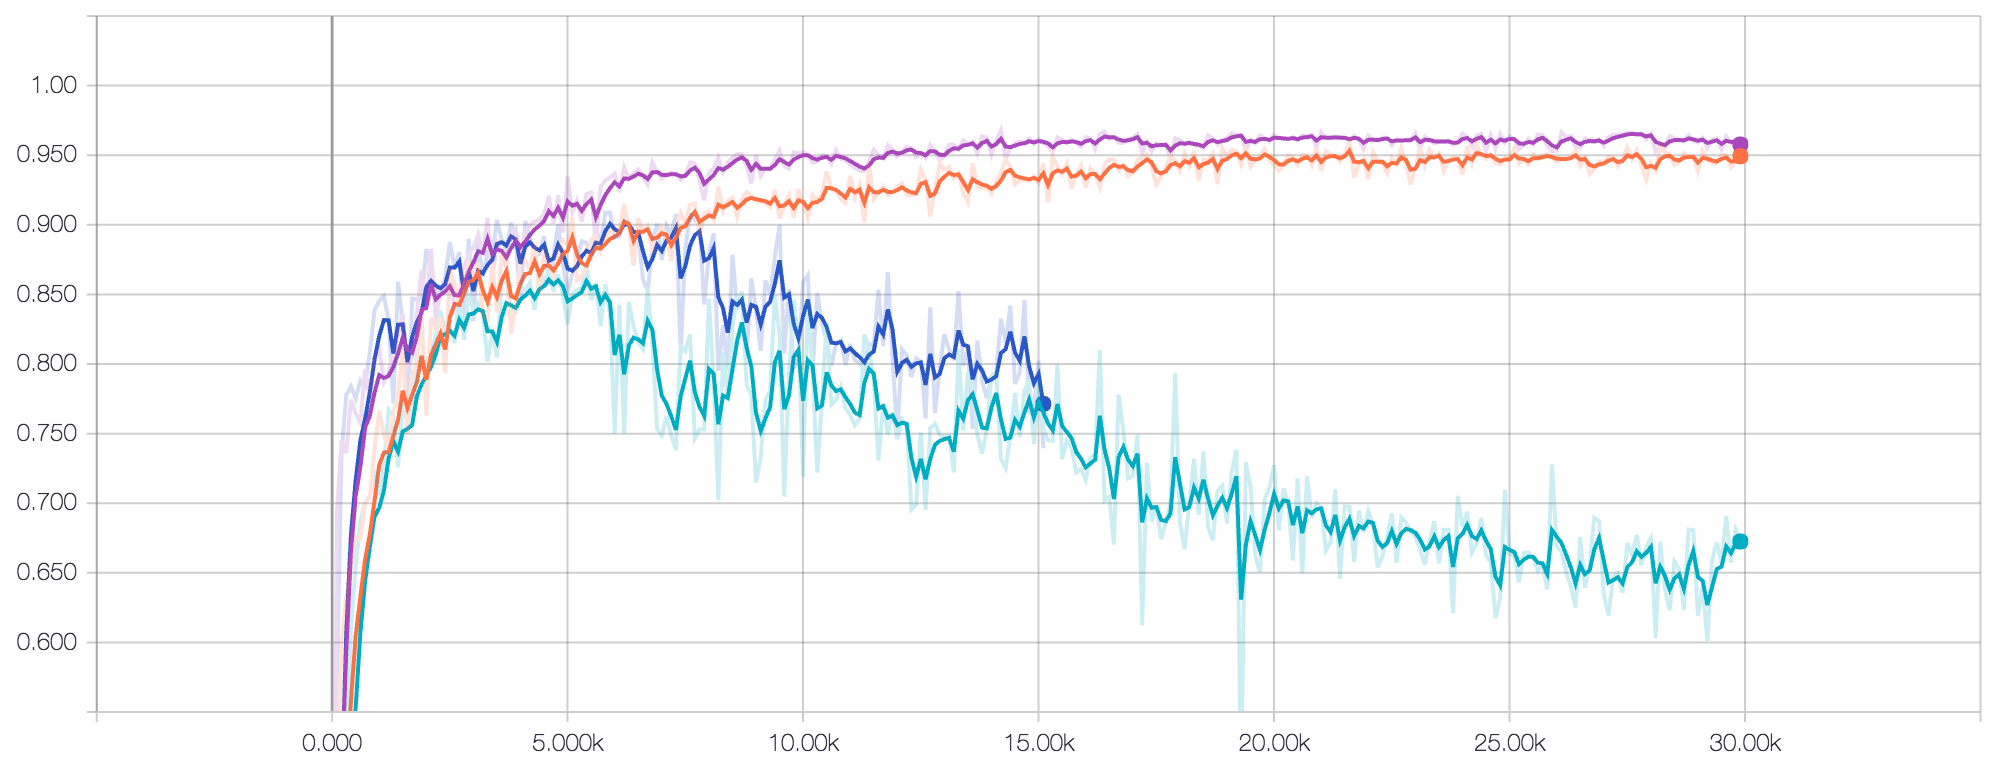
\includegraphics[width=\textwidth]{img/2d_rand.png} \\
\textbf{Pixel Error}
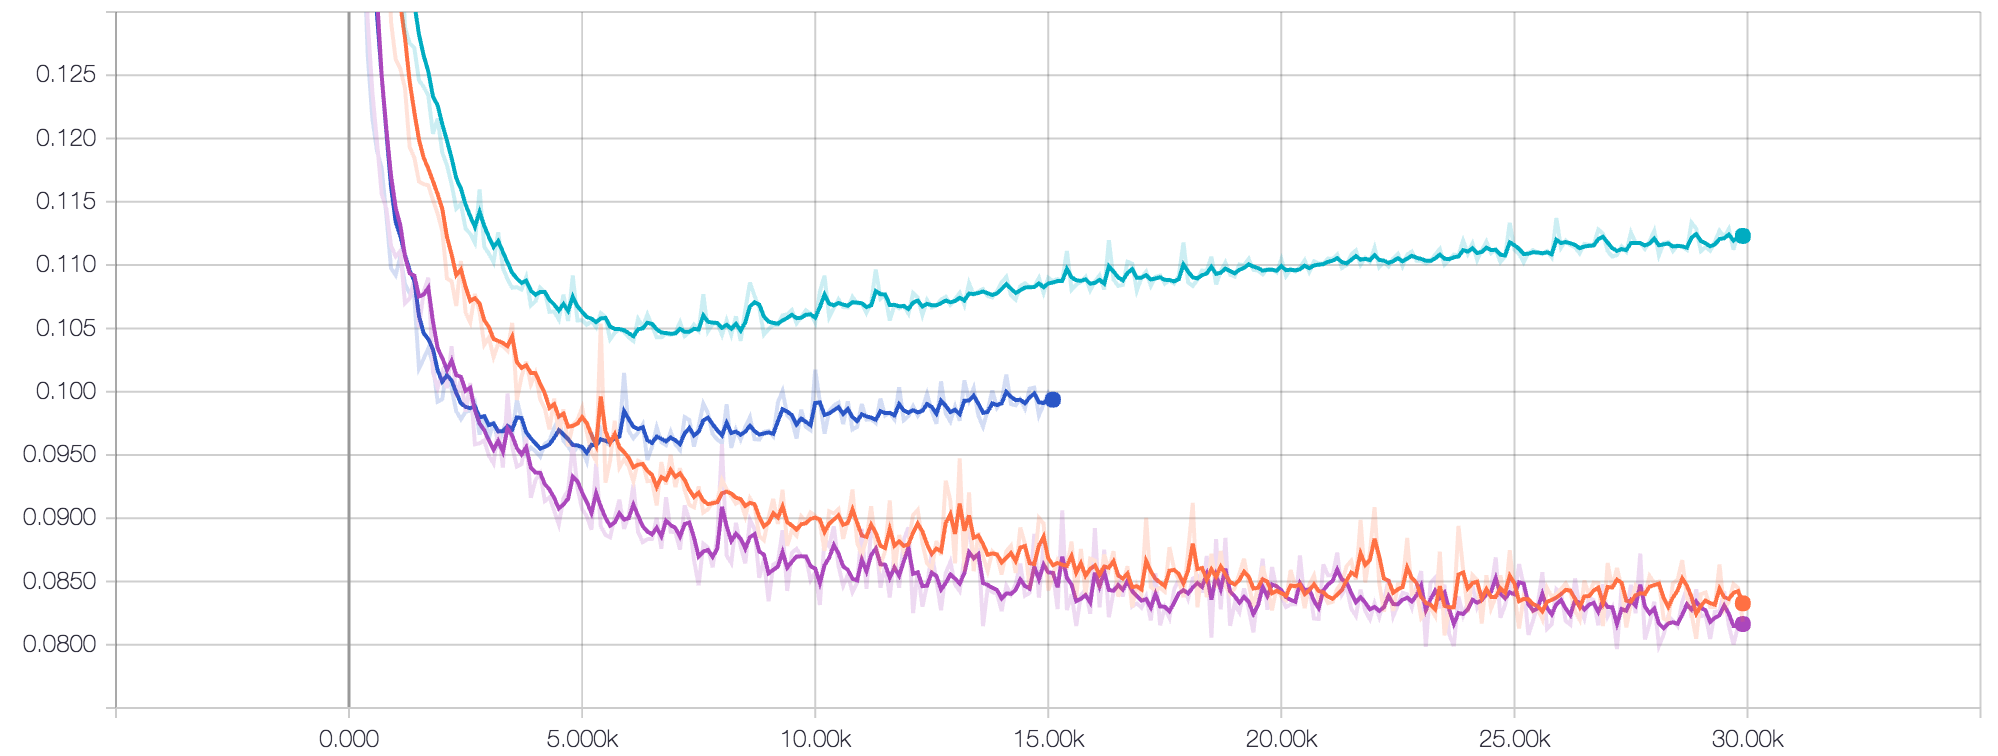
\includegraphics[width=\textwidth]{img/2d_pixel.png}
\label{fig:2d_training_curves}
\caption[Training curves for 2D segmentation]{Training curves, smoothed, for 2D segmentation. Top: The full Rand scores on the validation set (from top: VD2D, N4, VD2D w/o augmentation, N4 w/o augmentation). Bottom: The pixel error on the validation set (from top: N4 w/o augmentation, VD2D w/o augmentation, N4, VD2D).}

\end{figure}

Based on these results, we can draw three major conclusions. First, augmentation is extremely important in the training process. As the two graphs in Figure \ref{fig:2d_training_curves} demonstrate, models without random data augmentation learn for a short time, but they quickly begin to overfit, resulting in very poor generalization performance later on (even though the loss function continues to decrease). Second, we find that deeper nets can outperform shallower nets, since the deeper VD2D net outperforms the N4 architecture, which is a finding consistent with results of others who have used deep learning in segmentation tasks. Finally, we can conclude that these sorts of nets have a significant amount of variance in their predictions; by using ensembling methods we can reduce the variance between predictions, and thereby achieve higher performance. In later sections, we will explore further how training data quality affects training performance.